\section{Millimeter Wave Radar}
\label{section: background - millimeter wave radar}

Millimeter Wave Radars (mmWave radar) are a type of sensor which have been discussed for many decades already, with early research dating back to the 1970s and with commercial usage dating back to 1990 in the telecommunication sector, and the automotive industry starting to use it at the turn of the century \cite{menzel2008years}.
In recent years, mmWave radars have been used in a broad number of sensing applications, from human tracking and activity recognition, through to object inspection and classification \cite[Fig.~2]{vanberlo2021millimeter}.

This recent interest in mmWave-based sensing solutions over some of the alternative methods, such as lidar and camera-based sensing methods, is due to some of the inherent advantages present in mmWave-based systems.
% vs cameras
Cameras, for example, provide a detailed, high-resolution image of a specific location, but they are susceptible to environmental changes in the light intensity.
mmWave radars do not suffer from this limitation, since they are an active sensor, meaning that they observe the reflection of a signal which has been sent out by the sensor itself.
Furthermore, cameras do not usually include any information on the distance to an object, they simply produce a 2-D projection of the scene which is being sensed.
mmWave radars, on the other hand, provide a 3-D point cloud, which does have this range data.
% vs lidar
Many of these previously mentioned attributes are shared by both mmWave radars and lidar, a very important difference between these two methods, however, is the wavelength of light which is used in each system. 
Lidar (and other radio-frequency radars, for that matter) use a longer wavelength of light than mmWave radars.
This means that mmWave radars are able to produce results at a significantly higher resolution than other radar solutions, such as lidar \cite{yan2025advancements}.

\subsection{Workings}
\label{subsection: background - millimeter wave radar - workings}
% How do mmWave Radars work

% millimeter waves, and their advantages
Let us first discuss the working of these mmWave radars, as the name already implies, these sensors capture information about the world using electromagnetic radiation in the bandwidth between 30-300 GHz, or in other words, waves with a wavelength between 10-1 millimeter.
mmWave radars have a few distinct advantages because they use electromagnetic waves in this "millimeter wave" bandwidth.
The millimeter waves can, for example, pass through certain fabrics and materials which are opaque to most other sensors, such as cotton and leather \cite{meier2020propagation}, as well as materials such as plastic and wood \cite{kapilevich2011fmcw}.
This makes them ideas for detecting hidden objects, which can be essential in security circumstances.
Furthermore, this ability allows them to be seamlessly integrated into existing facades, creating a more seamless user experience.
The wavelength also allows mmWave radars to detect very small movements, "as small as a fraction of a millimeter" \cite[p.~2]{ti2020fundamentals}, this ability to sense very small changes is another advantage of the chosen bandwidth.

% Basic conceptual working
% mmWave radar sends a signal, it bounces back, and we get a pointcloud "like a bat".
Conceptually, the way in which mmWave radars "sense" the world around them is by sending out a signal (electromagnetic radiation) and observing the return signal, which has bounced off objects in the area to be observed.
In this way, the mmWave radar knows where these objects are, not all that dissimilar to how a bat senses, using echo location.
The distance to the object can be calculated using the time delay between sending the signal and receiving its echo.
By combining this distance with the direction from which the return signal came, the mmWave radar can specify a precise point in 3D space where "something" has been observed.
There are, however, a number of technical difficulties when it comes to making this theoretical system in the real world, the solutions to which will be discussed now.

% How the chirps work (mention FMCW)
% These millimeter waves are sent out as "chirps" by the system, which is why it's also called an FMCW
The mechanism by which an mmWave radar works relies on a few different ideas, which should first be covered.
Firstly, an important part of the mmWave radar is the \textit{chrip}.
mmWave radars sense by sending out a so-called \textit{chirp}, which is a signal of continuously increasing frequency (not unlike the chirps of some birds), which is visualized in \cref{fig:mmwave_chirp}, which is why these radars are also at times called \textit{Frequency Modulated Continuous Wave} (FMCW) radars.
% RX TX IF signal
Since this wave will travel for a certain amount of time before bouncing back to the sensor and being perceived again, it's found that the received return signal (\textbf{RX}) is a time delayed version of the transmitted signal (\textbf{TX}), where the exact time delay is dependent on the distance to the object which is to be observed.
This difference between the currently received signal and the currently transmitted signal's frequencies can be found by feeding both signals into a "mixer", a hardware device that can find the difference between the frequencies of two sine waves, and which will not be discussed in depth in this thesis.
Conceptually, this system is depicted in \cref{fig:mmwave_if_signal}
In this way, the mmWave radar can detect a distance as a time delay (using the known constant speed of light), without having to use any sort of timer, instead using some clever signal processing to get a value which is proportionately equal to the distance.
In reality, however, many such return signals will be generated by a variety of objects in the view window of the mmWave radar, thus, there will not be one singular IF signal, but rather the IF signal will contain multiple "tones", all representative of objects at different distances.
In reality, the system is even still a bit more complicated, but for the purposes of this thesis, this is in-depth enough. 
For a full explanation, please read \cite{introduction_to_mmwave}.


% Side-by-side figures 
\begin{figure}[h]
    \begin{minipage}[c]{0.4\textwidth}
    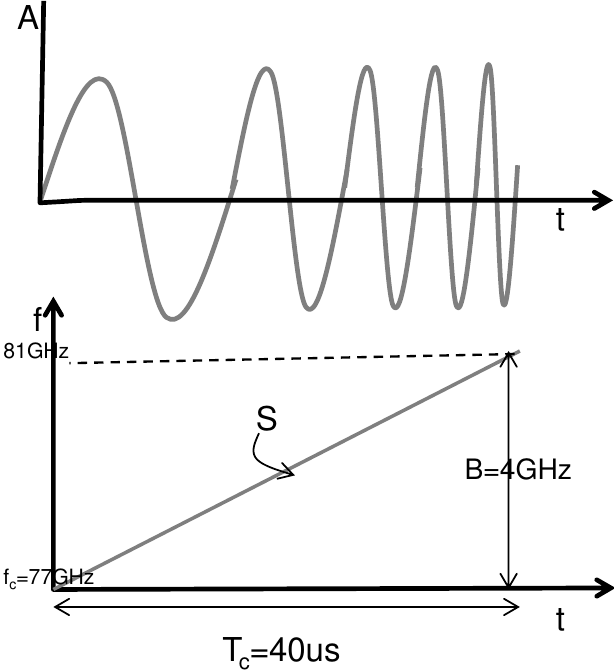
\includegraphics[width=\linewidth]{figures/mmwave/mmwave_chirp.png}
        \caption{Visualization of a "chirp". \cite{introduction_to_mmwave}}
        \label{fig:mmwave_chirp}
    \end{minipage}
    \hfill
    \begin{minipage}[c]{0.4\textwidth}
        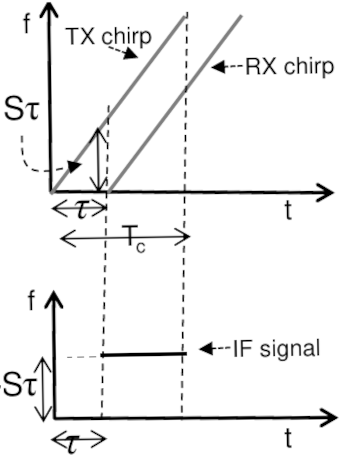
\includegraphics[width=\linewidth]{figures/mmwave/mmwave_IF_signal_cropped.png}
        \caption{The difference between RX and TX represents the distance. \cite{introduction_to_mmwave}}
        \label{fig:mmwave_if_signal}
    \end{minipage}%
\end{figure}


% Beam forming receiver principle
% A principle very similar to that of beam forming antennas is used to interpret this data.
In order to determine where the perceived object is, the mmWave radar needs to know the angle or arrival of the return signal.
For this, the mmWave uses an array of receiver antennas that are spaced half a wavelength apart, as shown in \cref{fig:mmwave_radar_antennas}. 
By measuring the difference in phase of the returned signal at each of the receiver antennas, the mmWave radar can infer from what lateral direction the signal came.
This is possible because, as the signal travels, the electromagnetic wave propagates, and its exact phase changes.
This phase can be detected by the mmWave radar, by using the previously mentioned "mixer", the specifics of which are not important to this thesis.
By comparing the phase of these two incoming signals, an angle can be derived, since the receivers are separated by a known distance, namely, half the wavelength ($\lambda$).
In a similar way, the mmWave radar can determine the elevation of an object by using the three transmitting antennas, since one of them is located with a slight vertical offset to the other two.

\begin{figure}[h]
    \begin{minipage}[c]{0.45\linewidth}
        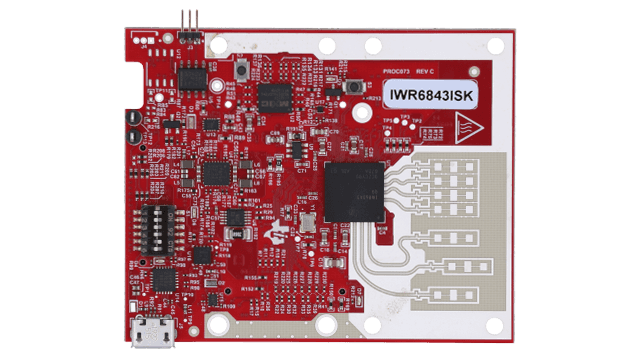
\includegraphics[width=0.95\linewidth]{figures/mmwave/iwr6843isk-top-sideways.png}
        \caption{Top down view of an IWR6843ISK MilliMeter Wave Radar}
        \label{fig:mmwave_radar_top_view}
    \end{minipage}
    \begin{minipage}[c]{0.45\linewidth}
        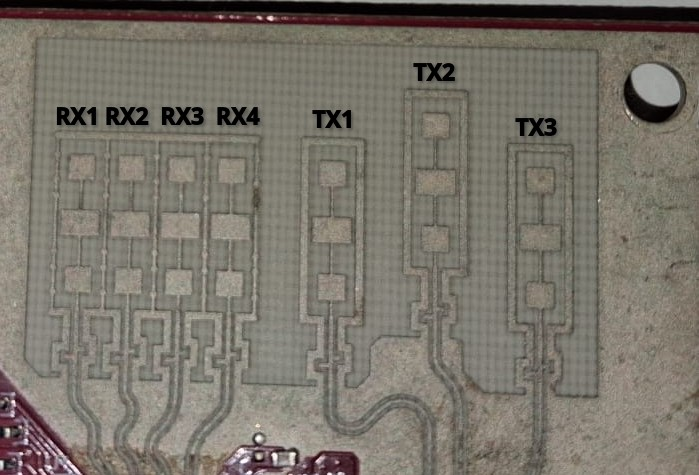
\includegraphics[width=0.95\linewidth]{figures/mmwave/WhatsApp Image 2025-10-28 at 15.59.05.jpeg}
        \caption{Antenna layout for the IWR6843ISK}
        \label{fig:mmwave_radar_antennas}
    \end{minipage}
\end{figure}

% 4 FFTs to get a pointcloud
% With a lot of FFTs, the data gets transformed from … to … to … to pointclouds.
The raw data being read by the mmWave radar is a complex waveform, comprised of many combined sinusoids, whose frequencies and phases are dependent on the objects being observed in the view of the radar.
The radar produces such a stream for each of its receiving antennas.
This data needs to be transformed to get useful information out of it, which is done by applying the \textit{Fourier Transformation} multiple times.
First, a Fourier Transform is used to convert this data from the \textit{time domain} to the \textit{frequency domain}, which should show the different distances at which objects have been observed, since the frequencies observed were dependent on the travel time of the mmWave.
Now this is done for a number of chirps, such that you can construct a matrix with the \textit{frequency domain} on one axis, and the \textit{chirp number} on the other, and another Fourier transform is considered, with regards to the \textit{chirp axis}, resulting in a \textit{range-velocity} matrix.
Lastly, the data from the different antennas is combined, giving a \textit{range-velocity-antenna} matrix. 
Suppose a Fourier transform is applied over this matrix, w.r.t. the antennas. 
In that case, the resulting matrix will be one of \textit{range-velocity-angle}, which can be interpreted as a point cloud.

\textbf{SIMPLIFY THE PART ABOVE}


\subsection{pointclouds}
\label{subsection: background - millimeter wave radar - pointclouds}
% Describe the pointclouds they generate, and some of their attributes (Doppler)

% What is a pointcloud
The output generated by the mmWave radar can vary somewhat, based on the firmware 
%(discussed in \cref{subsection: background - millimeter wave radar - configuration})
However, all firmware options do output \textit{point clouds}, in one representation or another.
In the case of mmWave radars, pointclouds are a collection of 4-dimensional vectors.
These vectors each have the 3 spatial dimensions, X, Y, and Z.
% Doppler
The last dimension is called the "Doppler" data, which is what, in the previous section, was called the "velocity".
This is done, as an object moving towards the sensor will increase the frequency of the millimeter wave by way of the Doppler effect, and likewise it will decrease the frequency if it's moving away.
In this way, the manner in which the velocity towards, and away from, the sensor is measured is by using the Doppler frequency shift that occurred.
This doppler information is quite unique to mmWave radars, since it provides a measure of how fast an object was moving at the moment a frame is captures, where most systems can only provide an estimation of the movement between frames.

% Characteristics of mmWave radar point clouds
There are many systems that generate pointclouds as an output, for example, lidar and RGBD cameras. 
It's thus important to look at the characteristics of pointclouds generated by mmWave radars.
One important way in which mmWave radars differ from these other systems is the high resolution that they can achieve, due to the wavelength used.
This allows mmWave radars to be used for various tasks that similar systems can't perform, such as the monitoring of vital signs, such as the heartbeat and respiratory rate \cite{wang2022heartprint, wang2023here} or systems which can reproduce audio, based on the vibrations of objects \cite{li2025acoustic, Lin2024highquality, Li2022mmphone}.
One disadvantage of mmWave radars, however, is that they produce very sparse pointclouds.
The experiments during this thesis have found that the mmWave Radar produces between 20-100 points per frame, at a rate of roughly 10 frames per second. 
This poses a significant challenge for any interpretation system, certainly those that try to interpret the mmWave radar point clouds in real time, with latency constraints.



% caveats and issues
During the design of IAmMuse, some issues with the mmWave radar point clouds were found, namely issues with noise and data stability.
Firstly, the noise, during this thesis, it was found that the mmWave radar is prone to producing high levels of noise due to reflections, the prevalence of this type of noise is also dependent on the specific environment in which the mmWave radar is used.
Besides this relatively regular environmental noise, noise spikes were also encountered semi-regularly during the use of the mmWave radar.
These noise spikes were often only present for one frame at a time, after which they disappeared again.
Another issue that was encountered was the distribution of points, namely, often a single frame would either hold points belonging to the right side of the user or points belonging to the left side of the user.
It's not clear if these issues were inherent to the chip we used, caused by misconfiguration, or caused by damage to the chip.


% \subsection{configuration}
% \label{subsection: background - millimeter wave radar - configuration}
% Texas Instruments provides several firmware setups \cite{ti_mmwave_firmware} for various of its mmWave radar chips, each implements separate interpretation methods over the raw data which is generated by the FMCW.

% Similar to lidar, mmWave radars are an active sensor, meaning that they do not rely on an external source of light, as they measure the reflection of a signal they send out themselves. 
% This means that they will work in any light situation, as opposed to cameras, which won't function properly if there is either too little or too much light.




% Give an explanation of what MMWave radars are, to what extent we can configure them, and what we get out of them (3d pointclouds, at ~10Hz, with between 30-100 points per frame).
% Mention the inherent privacy-preserving nature of MMWave due to its not capturing images, and how it fares better in varied light conditions (overexposure/underexposure).
% Also, briefly explain how they work internally, using \textit{beam forming antennas} on the receiving and, as well as the large amount of FFTs over the raw signal, to get to pointclouds.
% 


